% !TeX encoding = UTF-8
% !TeX spellcheck = en_US
% !TeX root = ../00_first_presentation.tex
\begin{frame}{KUKA youBot}

    The youBot is a mobile manipulator designed for education and research purposes. It comes with fully open interfaces and API. 
    \begin{columns}
    \begin{column}{8cm}
    %\begin{block}{System}
    		\begin{itemize}
    			\item Omnidirectional, four-wheeled
    			\item 5-DOF manipulator with a two-finger gripper
    			\item On-board PC with CPU, 2GB memory, 32GB SSD drive
    			\item Sensors: vision sensors, rangefinders
    		\end{itemize} 
    %\centering 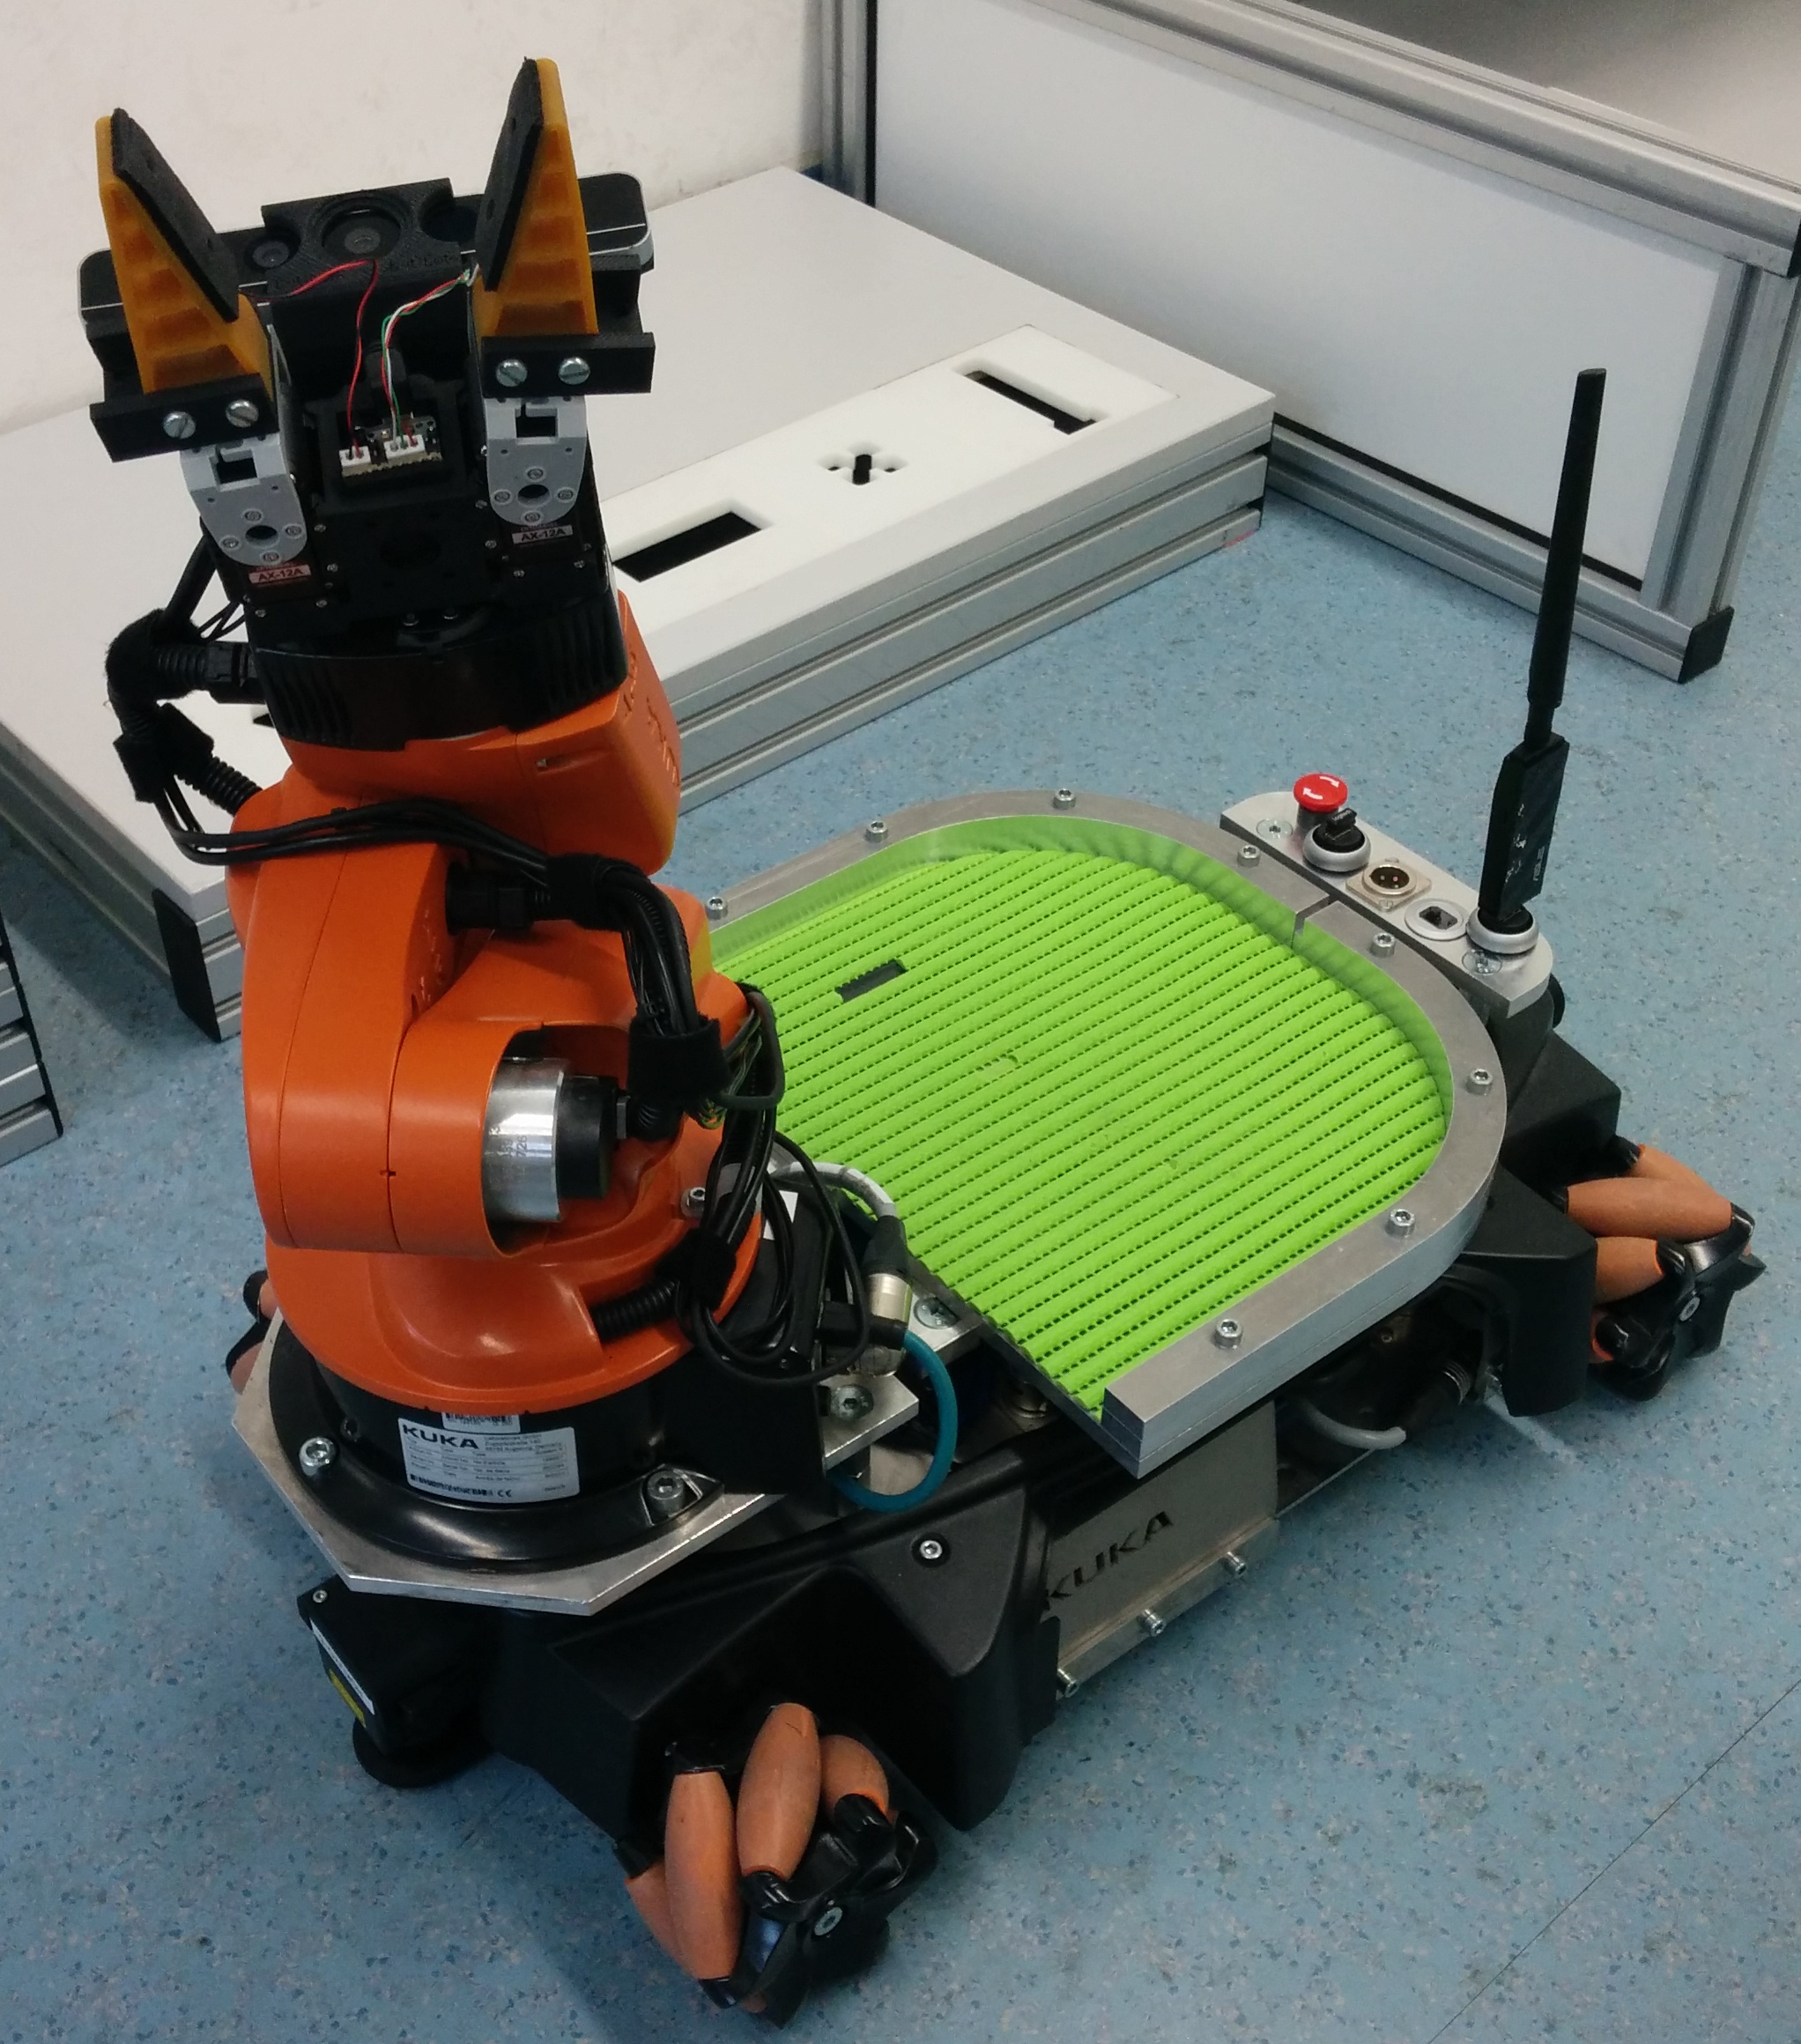
\includegraphics[width=0.25\textwidth]{slides/gfx/youbot.jpg}   
	%\end{block}
	\end{column}
	\begin{column}{5cm} % alternative top-align that's better for graphics
		\centering
    		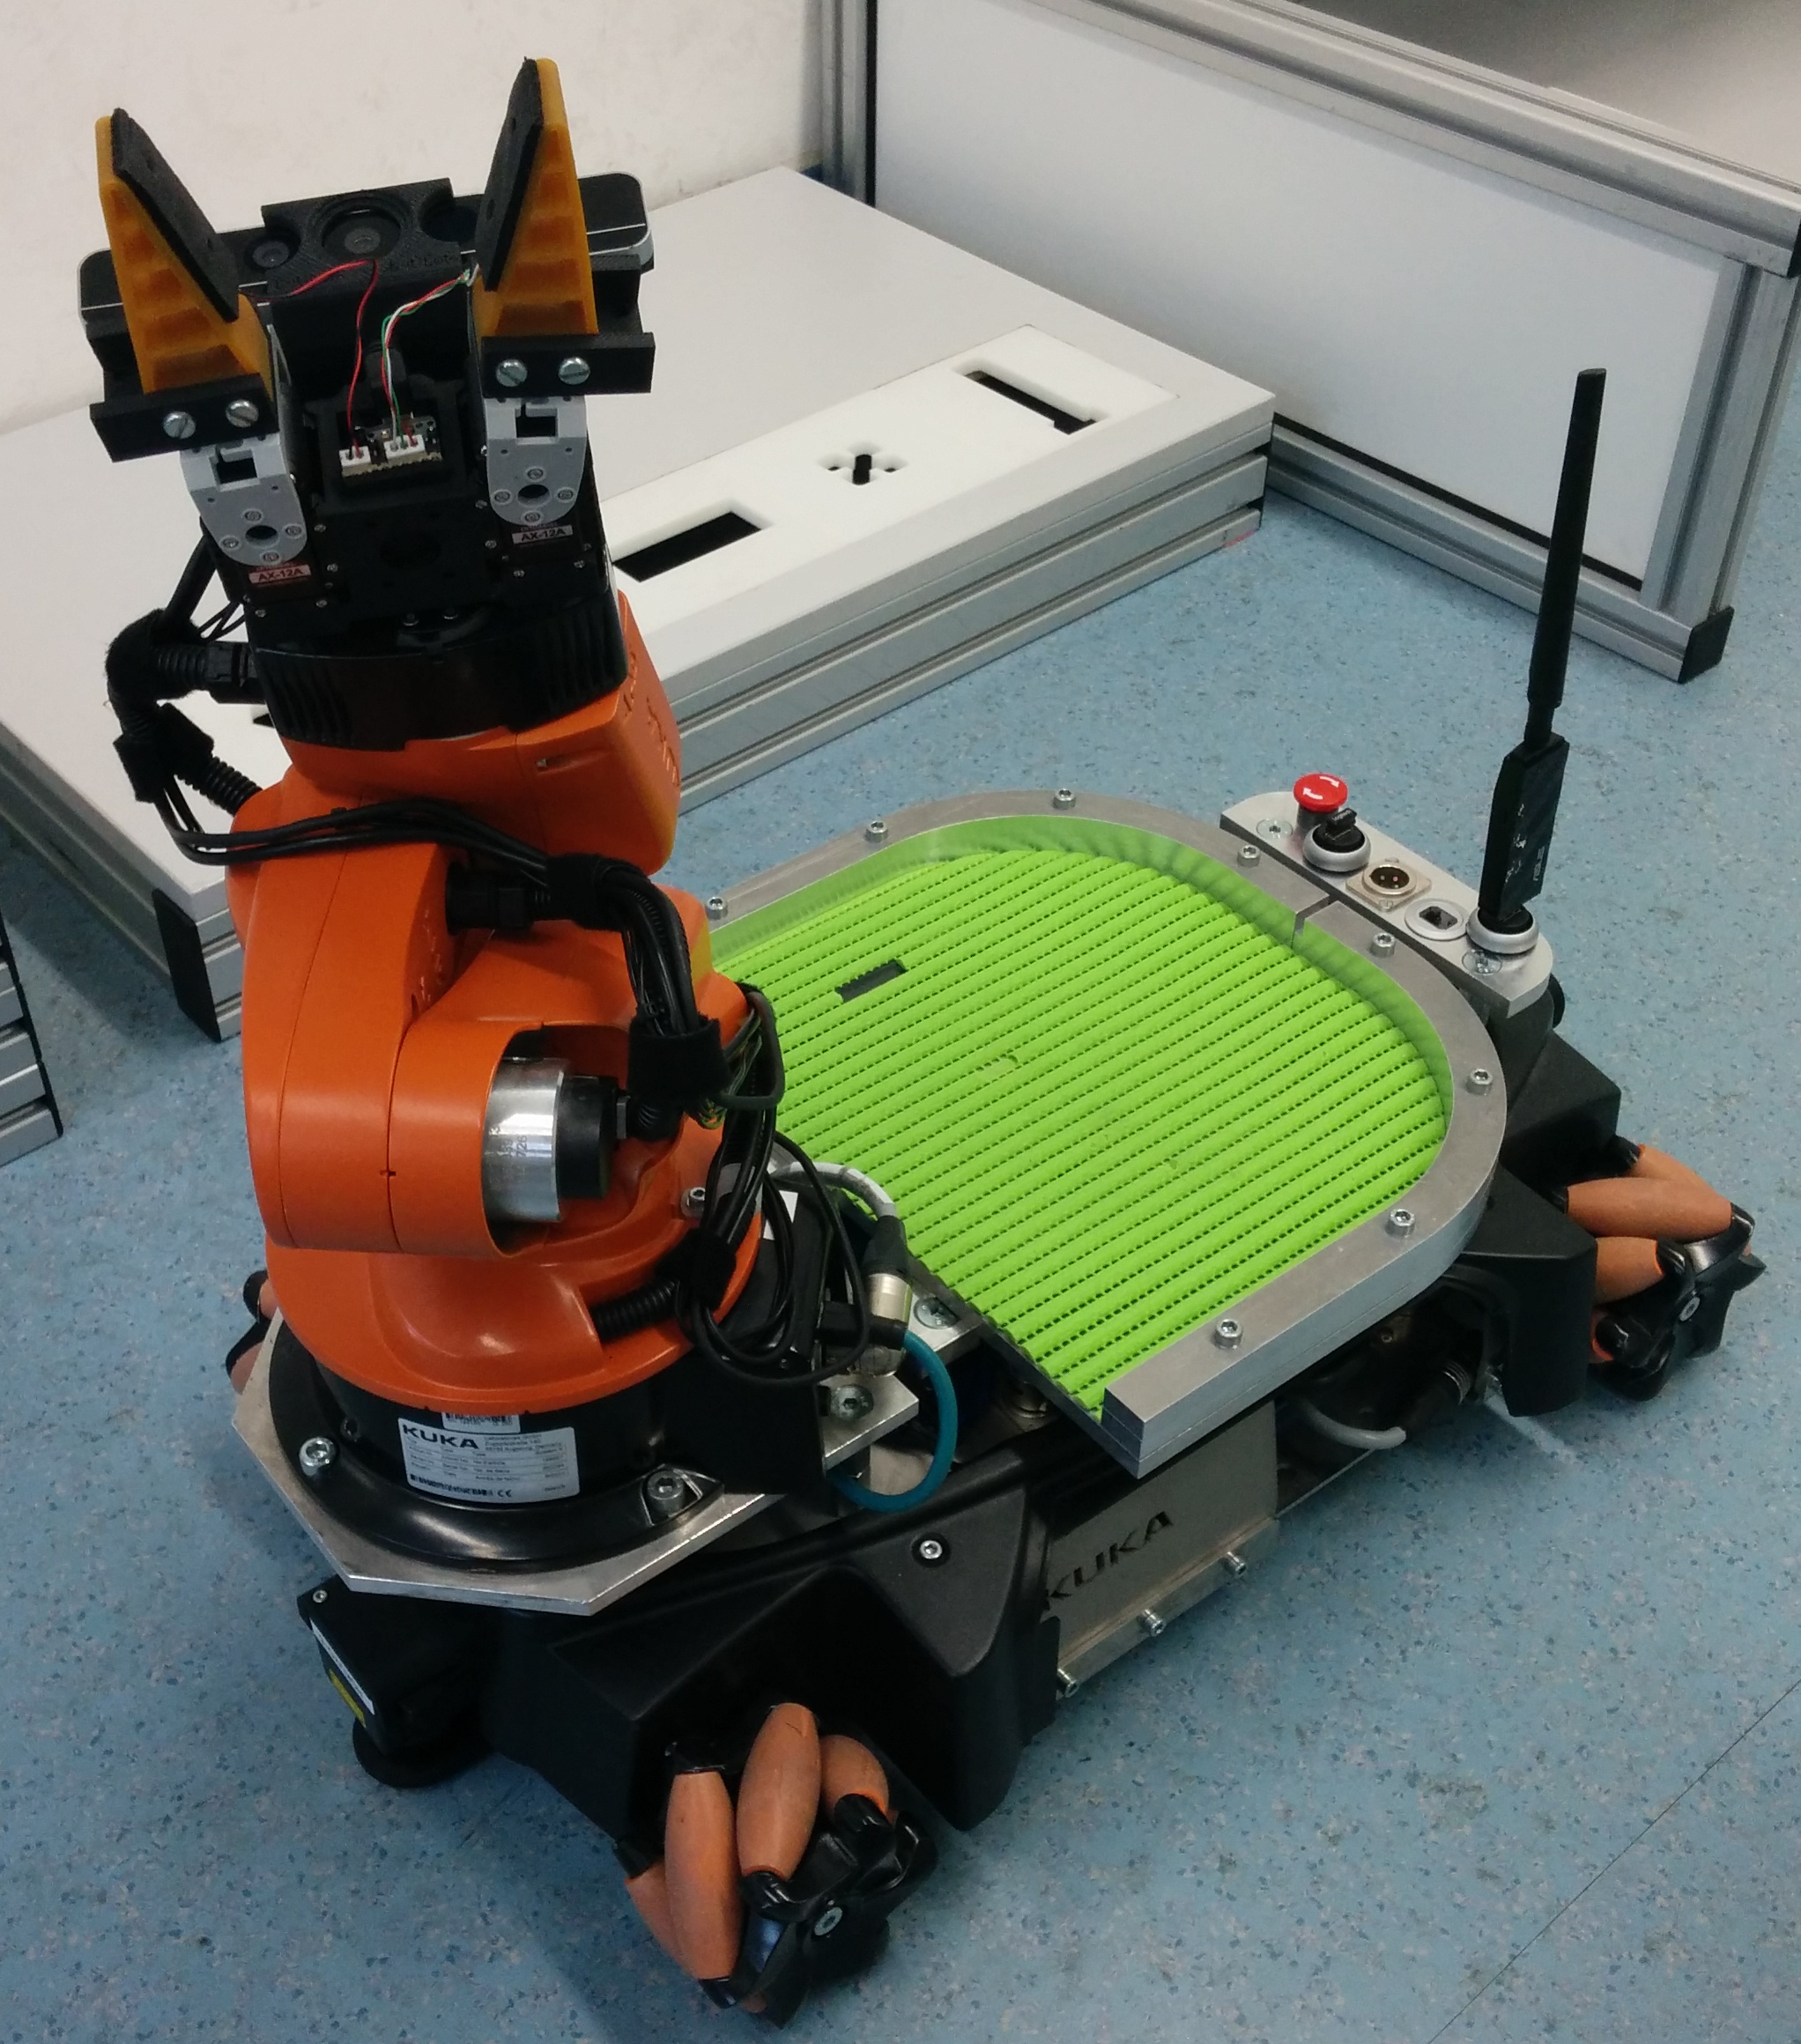
\includegraphics[height=50mm]{slides/gfx/youbot.jpg}
	\end{column}
	
	\end{columns}
\end{frame}
%---------------------------
%\begin{frame}{KUKA youBot}
    
    %\begin{itemize}
    		%\item Motor controllers of the wheels can be accessed via Ethernet and EtherCAT.
    		%\item I/O devices connection via USB and VGA 
    %\end{itemize}   

%\end{frame}
